\section{Redes Sem Fios (IEEE 802.11)}
\subsection*{Acesso Rádio}
\subsection{Identifique em que frequência do espectro está a operar a rede sem fios, e o canal que corresponde essa frequência.}

\begin{figure}[h]
    \centering
    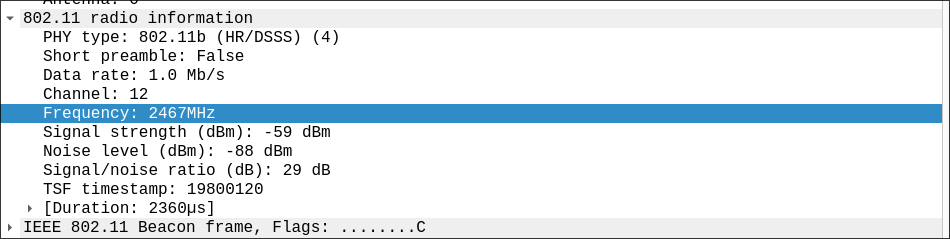
\includegraphics[width=0.8\textwidth]{freq.png}
    \caption{\label{fig:freq}Frequencia e channel de operacao da rede sem fios.}
\end{figure}

A rede sem fios está a operar na frequência de 2.467 GHz, e o canal que corresponde a essa frequência é o 12.

\subsection{Identifique a versão da norma IEEE 802.11 que está a ser usada.}

\begin{figure}[h]
    \centering
    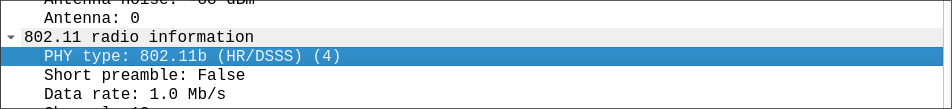
\includegraphics[width=0.8\textwidth]{ver.png}
    \caption{\label{fig:ver}Versao da norma IEEE 802.11, e data rate de operacao da rede sem fios.}
\end{figure}

A versao da norma IEEE 802.11 que está a ser usada é a 802.11b.

\subsection{Qual o débito a que foi enviada a trama escolhida? Será que esse débito  corresponde ao débito máximo a que a interface Wi-Fi pode operar? Justifique.}

Como pode ser observado na Figura \ref{fig:ver} o data rate de operacao da rede sem fios para a trama escolhida é de 1 Mb/s.

\begin{figure}[h]
    \centering
    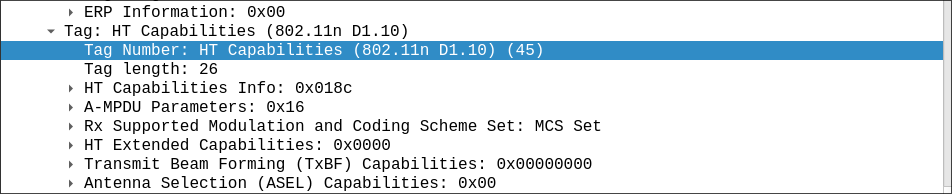
\includegraphics[width=0.8\textwidth]{ht.png}
    \caption{\label{fig:ht}Capacidade de operacao da rede sem fios.}
\end{figure}

\begin{figure}[h]
    \centering
    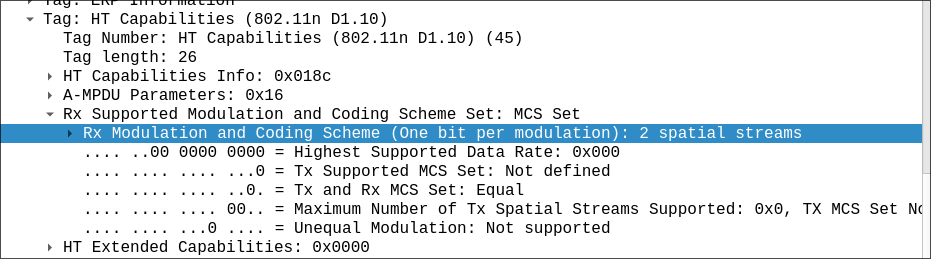
\includegraphics[width=0.8\textwidth]{channels.png}
    \caption{\label{fig:channels}Numero de Spatial Streams e canais de operacao da rede sem fios.}
\end{figure}

\begin{figure}[h]
    \centering
    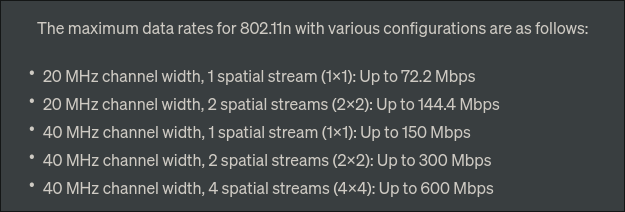
\includegraphics[width=0.8\textwidth]{chat.png}
    \caption{\label{fig:chat}Data rates de operacao da rede sem fios. (GPT-3.5)}
\end{figure}

De acordo com a HT Capabilities (Figura \ref{fig:ht}) a versao 802.11n é suportada, e
e de acordo com a Figura \ref{fig:channels} o numero de Spatial Streams é de 2, logo a data rate de operacao da rede sem fios pode variar de 144.4 Mbps a 300 Mbps conforme a Figura \ref{fig:chat}.

Logo o data rate de operacao da rede sem fios para a trama escolhida não corresponde ao débito máximo a que a interface Wi-Fi pode operar.

\subsection{Verifique qual a força do sinal (signal strength) e a qualidade expectável de  receção da trama, tendo em conta a tabela apresentada em Anexo.}

\begin{figure}[h]
    \centering
    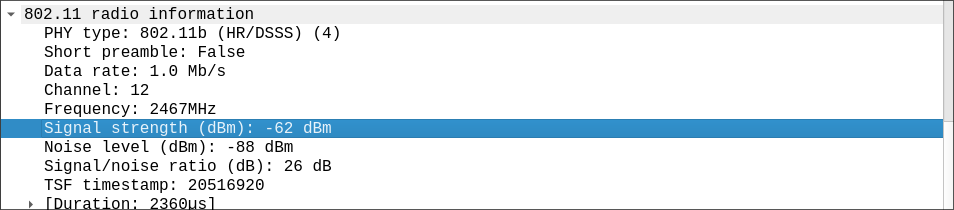
\includegraphics[width=0.8\textwidth]{signal.png}
    \caption{\label{fig:signal}Signal strength da trama.}
\end{figure}

De acordo com a signal strength de -62 dBm, a qualidade expectável de receção da trama é de "reliable signal strength (the edge of what is considered accurate to support Voice over WLAN)".

\subsection*{Scanning Passivo e Scanning Ativo}
\subsection{Selecione a trama beacon nr. 100+NG, sendo NG o seu número de grupo. Esta  trama pertence a que tipo de tramas 802.11? Indique o valor dos seus  identificadores de tipo e de subtipo. Em que parte concreta do cabeçalho da  trama estão especificados (ver anexo)?}

\begin{verbatim}
    No. Time Source Destination Protocol Length Info
    128 4.915351 HitronTe_af:b1:98 Broadcast 802.11 296 Beacon frame,
    SN=2179, FN=0, Flags=........C, BI=100, SSID="FlyingNet"

    Frame 128: 296 bytes on wire (2368 bits), 296 bytes captured (2368 bits)

    Radiotap Header v0, Length 25
    Header revision: 0
    Header pad: 0
    Header length: 25
    Present flags
    MAC timestamp: 24715251
    Flags: 0x10
    Data Rate: 1.0 Mb/s
    Channel frequency: 2467 [BG 12]
    Channel flags: 0x0480, 2 GHz spectrum, Dynamic CCK-OFDM
    Antenna signal: -65 dBm
    Antenna noise: -88 dBm
    Antenna: 0

    802.11 radio information
    PHY type: 802.11b (HR/DSSS) (4)
    Short preamble: False
    Data rate: 1.0 Mb/s
    Channel: 12
    Frequency: 2467MHz
    Signal strength (dBm): -65 dBm
    Noise level (dBm): -88 dBm
    Signal/noise ratio (dB): 23 dB
    TSF timestamp: 24715251
    [Duration: 2360µs]

    IEEE 802.11 Beacon frame, Flags: ........C
    Type/Subtype: Beacon frame (0x0008)
    Frame Control Field: 0x8000
    .000 0000 0000 0000 = Duration: 0 microseconds
    Receiver address: Broadcast (ff:ff:ff:ff:ff:ff)
    Destination address: Broadcast (ff:ff:ff:ff:ff:ff)
    Transmitter address: HitronTe_af:b1:98 (bc:14:01:af:b1:98)
    Source address: HitronTe_af:b1:98 (bc:14:01:af:b1:98)
    BSS Id: HitronTe_af:b1:98 (bc:14:01:af:b1:98)
    .... .... .... 0000 = Fragment number: 0
    1000 1000 0011 .... = Sequence number: 2179
    Frame check sequence: 0x4646c7af [unverified]
    [FCS Status: Unverified]

    IEEE 802.11 Wireless Management
    Fixed parameters (12 bytes)
    Timestamp: 1149675520479
    Beacon Interval: 0.102400 [Seconds]
    Capabilities Information: 0x0c31
    Tagged parameters (231 bytes)
    Tag: SSID parameter set: "FlyingNet"
    Tag: Supported Rates 1(B), 2(B), 5.5(B), 11(B), 9, 18, 36, 54, [Mbit/sec]
    Tag: DS Parameter set: Current Channel: 12
    Tag: Extended Supported Rates 6(B), 12(B), 24(B), 48, [Mbit/sec]
    Tag: Vendor Specific: Microsoft Corp.: WPS
    Tag: Traffic Indication Map (TIM): DTIM 1 of 3 bitmap
    Tag: ERP Information
    Tag: HT Capabilities (802.11n D1.10)
    Tag: HT Information (802.11n D1.10)
    Tag: Extended Capabilities (1 octet)
    Tag: Vendor Specific: Microsoft Corp.: WPA Information Element
    Tag: RSN Information
    Tag: Vendor Specific: Microsoft Corp.: WMM/WME: Parameter Element
    Tag: QBSS Load Element 802.11e CCA Version
    Tag: Vendor Specific: Ralink Technology, Corp.
\end{verbatim}

\begin{verbatim}
    IEEE 802.11 Beacon frame, Flags: ........C
    Type/Subtype: Beacon frame (0x0008)
    Frame Control Field: 0x8000
\end{verbatim}
A trama pertence ao tipo Beacon frame, e o valor dos seus identificadores de tipo e de subtipo são 0x0008 e 0x8000 respetivamente. Estes identificadores estão especificados no Frame Control Field da trama.

\subsection{Para a trama acima, identifique todos os endereços MAC em uso. Que conclui  quanto à sua origem e destino?}

\begin{verbatim}
    Receiver address: Broadcast (ff:ff:ff:ff:ff:ff)
    Destination address: Broadcast (ff:ff:ff:ff:ff:ff)
    Transmitter address: HitronTe_af:b1:98 (bc:14:01:af:b1:98)
    Source address: HitronTe_af:b1:98 (bc:14:01:af:b1:98)
    BSS Id: HitronTe_af:b1:98 (bc:14:01:af:b1:98)
\end{verbatim}

A origem é o Transmitter address, e o destino é o Receiver address, e o BSS Id é o identificador da rede sem fios, que é o mesmo que o Transmitter address.
A trama do tipo beacon é enviada periodicamente por um ponto de acesso (AP) ou por um nó de rede sem fios para anunciar a sua presença e disponibilidade, logo o Transmitter address é o endereço MAC do ponto de acesso (AP) ou do nó de rede sem fios, e o Receiver address é o endereço MAC de broadcast.

\subsection{Qual o intervalo de tempo previsto entre tramas beacon consecutivas?  (nota:  este valor é anunciado na própria trama beacon). Na prática, a periodicidade de  tramas beacon provenientes do mesmo AP é verificada com precisão? Justifique.}

\begin{verbatim}
    IEEE 802.11 Beacon frame, Flags: ........C
    Type/Subtype: Beacon frame (0x0008)
    Frame Control Field: 0x8000
    .000 0000 0000 0000 = Duration: 0 microseconds
    Receiver address: Broadcast (ff:ff:ff:ff:ff:ff)
\end{verbatim}

O intervalo de tempo previsto entre tramas beacon consecutivas é de 0 microsegundos, ou seja, as tramas beacon são enviadas continuamente.
Na pratica, a periodicidade de tramas beacon nao e verificada com precisao.

\subsection{Identifique e liste os SSIDs dos APs que estão a operar na vizinhança da STA de  captura? Explicite o modo como obteve essa informação (por exemplo, se usou  algum filtro para o efeito).}

O filtro usado no wireshark para obter os SSIDs dos APs que estão a operar na vizinhança da STA de captura foi o seguinte: \(wlan.fc.type\_subtype == 8\).

\begin{figure}
    \centering
    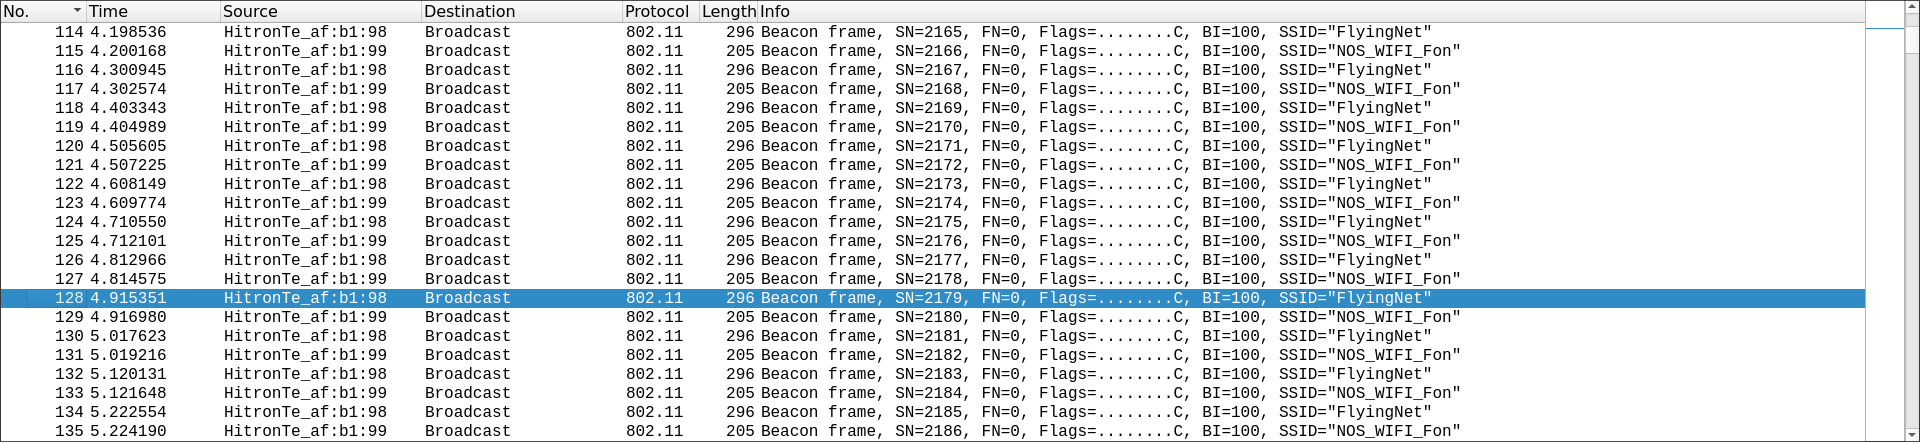
\includegraphics[width=0.8\textwidth]{ssids.png}
    \caption{\label{fig:ssids}SSIDs dos APs que estão a operar na vizinhança da STA de captura.}
\end{figure}

A lista dos SSIDs dos APs que estão a operar na vizinhança da STA de captura é a seguinte:
\begin{itemize}
    \item FlyingNet
    \item NOS\_WIFI\_Fon
\end{itemize}

\end{document}